\section{Spark::Sp\-Stream\-Output Class Reference}
\label{classSpark_1_1SpStreamOutput}\index{Spark::SpStreamOutput@{Spark::SpStreamOutput}}
{\tt \#include $<$Sp\-Stream\-Output.h$>$}

Inheritance diagram for Spark::Sp\-Stream\-Output:\begin{figure}[H]
\begin{center}
\leavevmode
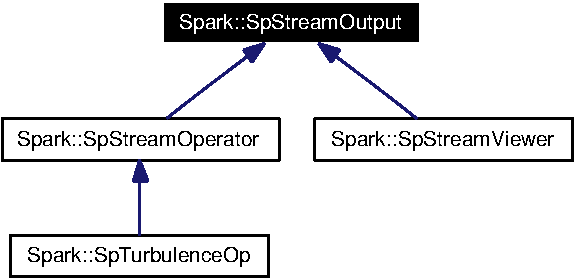
\includegraphics[width=155pt]{classSpark_1_1SpStreamOutput__inherit__graph}
\end{center}
\end{figure}
Collaboration diagram for Spark::Sp\-Stream\-Output:\begin{figure}[H]
\begin{center}
\leavevmode
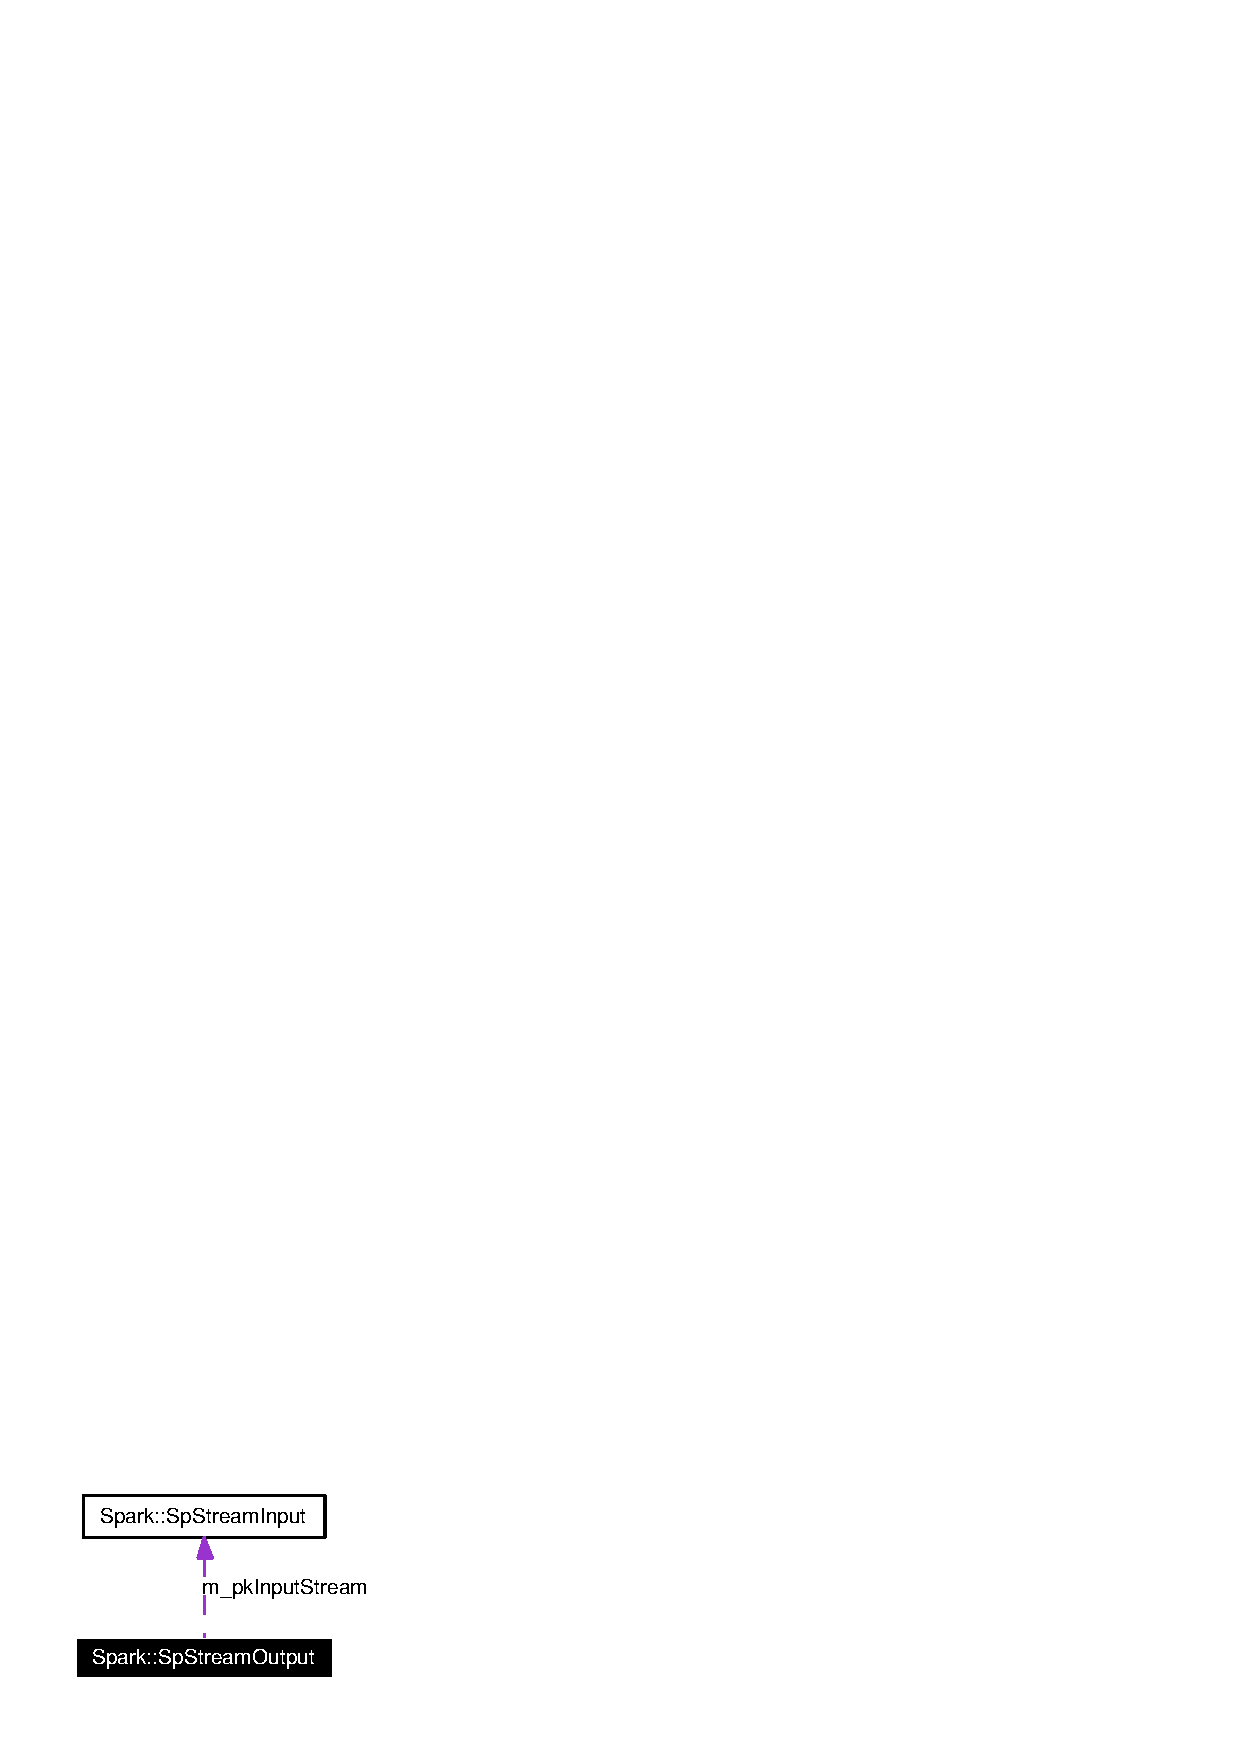
\includegraphics[width=90pt]{classSpark_1_1SpStreamOutput__coll__graph}
\end{center}
\end{figure}


\subsection{Detailed Description}
Abstract base class for an output stream used fo saving/viewing stream data. 

Definition at line 32 of file Sp\-Stream\-Output.h.\subsection*{Public Member Functions}
\begin{CompactItemize}
\item 
{\bf Sp\-Stream\-Output} ()
\begin{CompactList}\small\item\em Construction:. \item\end{CompactList}\item 
virtual {\bf $\sim$Sp\-Stream\-Output} ()
\item 
virtual void {\bf set\-Input\-Stream} ({\bf Sp\-Stream\-Input} $\ast$pk\-Input\-Stream)
\begin{CompactList}\small\item\em Sets the current source operator. \item\end{CompactList}\end{CompactItemize}
\subsection*{Protected Attributes}
\begin{CompactItemize}
\item 
{\bf Sp\-Stream\-Input} $\ast$ {\bf m\_\-pk\-Input\-Stream}
\begin{CompactList}\small\item\em Internal Data:. \item\end{CompactList}\item 
bool {\bf m\_\-b\-Has\-Changed}
\end{CompactItemize}


\subsection{Constructor \& Destructor Documentation}
\index{Spark::SpStreamOutput@{Spark::Sp\-Stream\-Output}!SpStreamOutput@{SpStreamOutput}}
\index{SpStreamOutput@{SpStreamOutput}!Spark::SpStreamOutput@{Spark::Sp\-Stream\-Output}}
\subsubsection{\setlength{\rightskip}{0pt plus 5cm}Spark::Sp\-Stream\-Output::Sp\-Stream\-Output ()\hspace{0.3cm}{\tt  [inline]}}\label{classSpark_1_1SpStreamOutput_a0}


Construction:. 

Definition at line 38 of file Sp\-Stream\-Output.h.

References m\_\-b\-Has\-Changed, and m\_\-pk\-Input\-Stream.\index{Spark::SpStreamOutput@{Spark::Sp\-Stream\-Output}!~SpStreamOutput@{$\sim$SpStreamOutput}}
\index{~SpStreamOutput@{$\sim$SpStreamOutput}!Spark::SpStreamOutput@{Spark::Sp\-Stream\-Output}}
\subsubsection{\setlength{\rightskip}{0pt plus 5cm}virtual Spark::Sp\-Stream\-Output::$\sim${\bf Sp\-Stream\-Output} ()\hspace{0.3cm}{\tt  [inline, virtual]}}\label{classSpark_1_1SpStreamOutput_a1}


Definition at line 45 of file Sp\-Stream\-Output.h.

\subsection{Member Function Documentation}
\index{Spark::SpStreamOutput@{Spark::Sp\-Stream\-Output}!setInputStream@{setInputStream}}
\index{setInputStream@{setInputStream}!Spark::SpStreamOutput@{Spark::Sp\-Stream\-Output}}
\subsubsection{\setlength{\rightskip}{0pt plus 5cm}virtual void Spark::Sp\-Stream\-Output::set\-Input\-Stream ({\bf Sp\-Stream\-Input} $\ast$ {\em pk\-Input\-Stream})\hspace{0.3cm}{\tt  [inline, virtual]}}\label{classSpark_1_1SpStreamOutput_a2}


Sets the current source operator. 



Reimplemented in {\bf Spark::Sp\-Stream\-Operator} {\rm (p.\,\pageref{classSpark_1_1SpStreamOperator_a2})}, and {\bf Spark::Sp\-Turbulence\-Op} {\rm (p.\,\pageref{classSpark_1_1SpTurbulenceOp_a4})}.

Definition at line 54 of file Sp\-Stream\-Output.h.

References m\_\-b\-Has\-Changed, and m\_\-pk\-Input\-Stream.

\subsection{Member Data Documentation}
\index{Spark::SpStreamOutput@{Spark::Sp\-Stream\-Output}!m_bHasChanged@{m\_\-bHasChanged}}
\index{m_bHasChanged@{m\_\-bHasChanged}!Spark::SpStreamOutput@{Spark::Sp\-Stream\-Output}}
\subsubsection{\setlength{\rightskip}{0pt plus 5cm}bool {\bf Spark::Sp\-Stream\-Output::m\_\-b\-Has\-Changed}\hspace{0.3cm}{\tt  [protected]}}\label{classSpark_1_1SpStreamOutput_p1}


Definition at line 64 of file Sp\-Stream\-Output.h.

Referenced by set\-Input\-Stream(), and Sp\-Stream\-Output().\index{Spark::SpStreamOutput@{Spark::Sp\-Stream\-Output}!m_pkInputStream@{m\_\-pkInputStream}}
\index{m_pkInputStream@{m\_\-pkInputStream}!Spark::SpStreamOutput@{Spark::Sp\-Stream\-Output}}
\subsubsection{\setlength{\rightskip}{0pt plus 5cm}{\bf Sp\-Stream\-Input}$\ast$ {\bf Spark::Sp\-Stream\-Output::m\_\-pk\-Input\-Stream}\hspace{0.3cm}{\tt  [protected]}}\label{classSpark_1_1SpStreamOutput_p0}


Internal Data:. 

Definition at line 63 of file Sp\-Stream\-Output.h.

Referenced by set\-Input\-Stream(), and Sp\-Stream\-Output().

The documentation for this class was generated from the following file:\begin{CompactItemize}
\item 
{\bf Sp\-Stream\-Output.h}\end{CompactItemize}
